\documentclass{article}


\usepackage[margin=1in]{geometry}
\usepackage{amsmath}
\usepackage{graphicx}
\usepackage{tabu}
\usepackage{listings}
\usepackage{color}
\usepackage{float}
\usepackage{caption}
\usepackage{subcaption}

\author{Zachary Vogel}
\title{Numerical Analysis Homework 5\\ APPM 4650}
\date{\today}

\begin{document}

\definecolor{keywords}{RGB}{255,0,90}
\definecolor{comments}{RGB}{0,0,113}
\definecolor{red}{RGB}{160,0,0}
\definecolor{green}{RGB}{0,150,0}
 
\lstset{language=Python, basicstyle=\ttfamily\small, keywordstyle=\color{keywords}, commentstyle=\color{comments},stringstyle=\color{red},showstringspaces=false,identifierstyle=\color{green}}



\maketitle


\section*{Problem 1}
Here we consider:
\[\begin{pmatrix}4 & 3 & 0\\3 & 4&-1\\0&-1&4\end{pmatrix}\begin{pmatrix}x_1\\x_2\\x_3\end{pmatrix}=\begin{pmatrix}24\\30\\-24\end{pmatrix}\]
Solve this system of equations using Gauss-Seidel with relaxation. Determine the optimum relaxation factor $\omega$ where $x_{i+1}=x_i+\omega\frac{r_i}{a_{ii}}$ to get the solution within 6 decimal places.\\
Here, I found the optimal relaxation factor to be $1.25$. The iterative solutions to this problem can be seen below, and the code in the Appendix 1.
\begin{figure}[H]
    \centering
    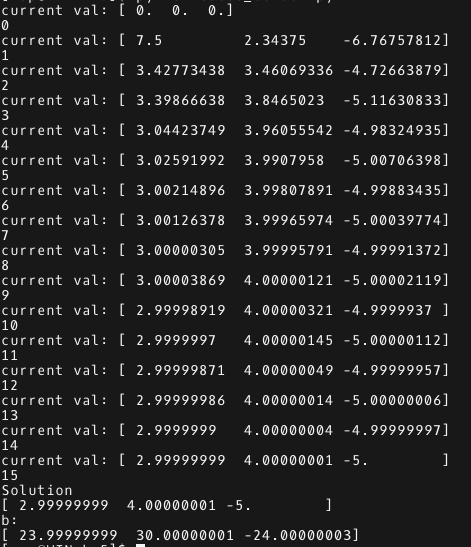
\includegraphics[width=0.6\textwidth]{p1.png}
\end{figure}

\section*{Problem 2}
Consider the matrix:
\[A=\begin{pmatrix}3&0&1\\0&5&0\\-1&1&-1\end{pmatrix}\]

\subsection*{(a)}
Calculate $A^{-1}$ exactly using the cofactor method.\\
The output of my script that calculated this is below, the code is in appendix 2.
\begin{figure}[H]
    \centering
    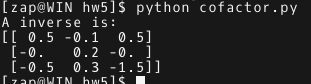
\includegraphics[width=0.6\textwidth]{p21a.png}
\end{figure}

\subsection*{(b)}
Start with the inital approximation to $A^{-1}$ of:
\[x_0=\begin{pmatrix}0.5&-0.1&0.4\\0&0.2&0\\-0.4&0.3&-1.5\end{pmatrix}\]
and use the iterative method $x_{i+1}=x_i(2I-Ax_i)$ to calculate the next approximation $x_1$.\\
The solution produced by my code can be seen below, the code is in appendix 2.
\begin{figure}[H]
    \centering
    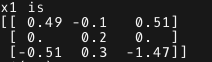
\includegraphics[width=0.6\textwidth]{p2a.png}
\end{figure}
\subsection*{(c)}
Calculate the deviations of $x_0$ and $x_1$ from the true inverse matrix $A^{-1}$.\\
The actual inverse is:
\[A^{-1}=\begin{pmatrix}0.5&-0.1&0.5\\0&0.2&0\\-0.5&0.3&-1.5\end{pmatrix}\]
The deviations can be seen below:
\begin{figure}[H]
    \centering
    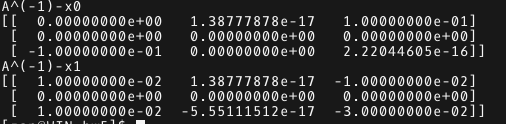
\includegraphics[width=0.8\textwidth]{p2b.png}
\end{figure}

\section*{Problem 3}
Use the power method to find the dominant eigenvalue $\lambda$ and the corresponding eigenvector $V$ for the matrix:
\[A=\begin{pmatrix}2&-1&0&0\\-1&2&-1&0\\0&-1&2&-1\\0&0&-1&2\end{pmatrix}\]

\subsection*{(a)}
Start the procedure with the initial vector $x_0=(1,1,1,1)^T$.\\
It's interesting that this converged to the second largest eigenvalue. The code is in appendix 3, the output can be seen below.
\begin{figure}[H]
    \centering
    \begin{subfigure}[b]{0.5\textwidth}
        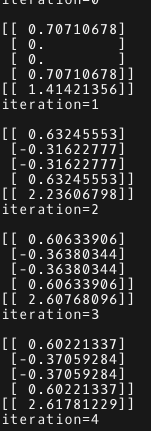
\includegraphics[width=0.5\textwidth]{p3a.png}
    \end{subfigure}
    \begin{subfigure}[b]{0.49\textwidth}
        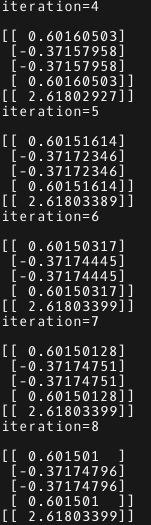
\includegraphics[width=0.5\textwidth]{p3a1.png}
    \end{subfigure}
\end{figure}


\subsection*{(b)}
Now, repeat the calculations starting with $x_0=(1,1,5,1)^T$.\\
Again, the output is below, code in appendix 3.
\begin{figure}[H]
    \centering
    \begin{subfigure}[b]{0.5\textwidth}
        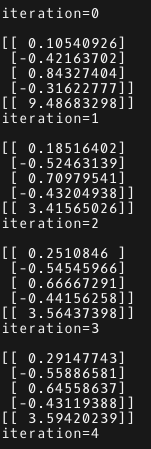
\includegraphics[width=0.5\textwidth]{p3b1.png}
    \end{subfigure}
    \begin{subfigure}[b]{0.49\textwidth}
        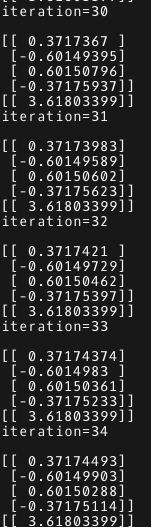
\includegraphics[width=0.5\textwidth]{p3b2.png}
    \end{subfigure}
\end{figure}
\subsection*{(c)}
Commment on the results from parts (a) and (b).

\section*{Problem 4}
Consider the matrix and initial vector:
\[A=\begin{pmatrix}2 & -1 & 1\\-1&3&2\\1&2&3\end{pmatrix}\quad x_0=\begin{pmatrix}1\\1\\1\end{pmatrix}\]

\subsection*{(a)}
Calculate the Rayleigh quotient and the error estimate using $x_2$ and $x_3$.\\
Didn't know how to do the error estimate, but the first few values can be seen below. Code is in appendix 4.
\begin{figure}[H]
    \centering
    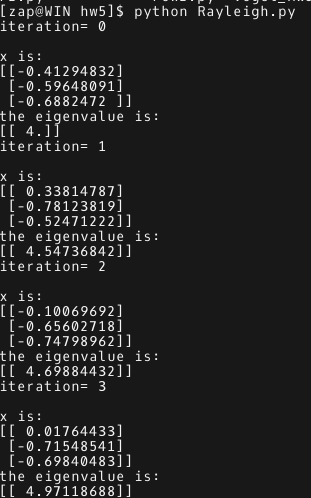
\includegraphics[width=0.5\textwidth]{p4a.png}
\end{figure}

\subsection*{(b)}
Use the power method to find $\lambda_{\text{max}}$ and the corresponding $V_{\text{max}}$.\\
Values can be seen below, code is in appendix 4.
\begin{figure}[H]
    \centering
    \begin{subfigure}[b]{0.49\textwidth}
        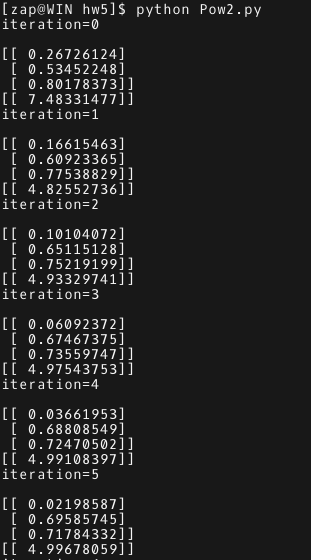
\includegraphics[width=0.8\textwidth]{p4b1.png}
    \end{subfigure}
    \begin{subfigure}[b]{0.49\textwidth}
        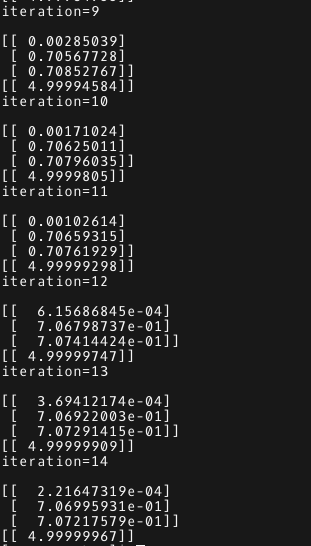
\includegraphics[width=0.8\textwidth]{p4b2.png}
    \end{subfigure}
\end{figure}


\clearpage
\appendix
\section{Appendix 1}
\lstinputlisting{Gauss_Seidel.py}


\section{Appendix 2}
\lstinputlisting{cofactor.py}
\lstinputlisting{P2.py}


\section{Appendix 3}
\lstinputlisting{Pow1.py}

\section{Appendix 4}
\lstinputlisting{Rayleigh.py}
\lstinputlisting{Pow2.py}
\end{document}
